%% AMS-LaTeX Created with the Wolfram Language : www.wolfram.com

\documentclass{article}
\usepackage{amsmath, amssymb, graphics, setspace}

\newcommand{\mathsym}[1]{{}}
\newcommand{\unicode}[1]{{}}

\newcounter{mathematicapage}
\begin{document}

\title{Penrose Encoding and graph visualization.}
\author{\\
Diana Itzel V{\' a}zquez Santiago.\\
Emmanuel Isaac Ju{\' a}rez Caballero.\\
Jes{\' u}s Eduardo Hermosilla D{\' \i}az.\\
Maestr{\' \i}a en Inteligencia Artificial, generaci{\' o}n 2021-2023}
\date{}
\maketitle

\begin{doublespace}
\noindent\(\pmb{\text{(*Starting Executing Cells*)}}\\
\pmb{\text{Clear}[\text{{``}Global$\grave{ }$*{''}}];}\\
\pmb{\text{SetDirectory}[\text{NotebookDirectory}[]];}\\
\pmb{\text{FindExternalEvaluators}[\text{{``}Python{''}}]}\\
\pmb{\text{session}=\text{StartExternalSession}[\text{{``}Python{''}}]}\)
\end{doublespace}

\begin{doublespace}
\noindent\(\pmb{u=\text{Import}[\text{{``}nuniversal.txt{''}}]\text{//}\text{ToExpression};}\\
\pmb{\text{n1}=450813704461563958982113775643437908;}\\
\pmb{\text{n2}=10389728107;}\\
\pmb{n=u;}\\
\pmb{\text{ExternalEvaluate}[\text{session},\text{File}[\text{{``}penrose$\_$encoding.py{''}}]];}\\
\pmb{\text{PenroseEncoding}=\text{ExternalEvaluate}[\text{session},\text{{``}codificacion{''}}];}\\
\pmb{\text{execution}=\text{PenroseEncoding}[\text{n2}];}\)
\end{doublespace}

\noindent\(\text{TM after Penrose Coding:  R10R1R100R111RR1H}\)

\noindent\(\text{  Instructions from TM}\)

\noindent\(\text{0            00 -$>$ 00R}\)

\noindent\(\text{1            01 -$>$ 10R}\)

\noindent\(\text{2            10 -$>$ 01R}\)

\noindent\(\text{3           11 -$>$ 100R}\)

\noindent\(\text{4          100 -$>$ 111R}\)

\noindent\(\text{5           101 -$>$ 00R}\)

\noindent\(\text{6           110 -$>$ 01H}\)

\begin{doublespace}
\noindent\(\pmb{\text{MT}=\text{Import}[\text{{``}universal.txt{''}}];}\)
\end{doublespace}

\begin{doublespace}
\noindent\(\pmb{\text{MT}=\text{StringDelete}[\text{StringSplit}[\text{Text}[\text{MT}][[1]],\text{{``},{''}}],\{\text{{``}[{''}},\text{{``}]{''}},\text{{``}'{''}},
\text{{``} {''}}\}];}\)
\end{doublespace}

\subsection*{MultiGraph2 implementation: A tool to visualize correctly multilabel graphs on Wolfram Mathematica}

\begin{doublespace}
\noindent\(\pmb{\text{ClearAll}[\text{multiGraph2}]}\\
\pmb{\text{multiGraph2}[\text{vl$\_$},\text{elist$\_$},\text{elabels$\_$},\text{estyles$\_$},o:\text{OptionsPattern}[\text{Graph}]]\text{:=}}\\
\pmb{\text{Module}[\{\text{esf},\text{edges},\text{labels},\text{styles},\text{sorted}=\text{Transpose}@\text{SortBy}[\text{Transpose}[\{\text{elist},\text{elabels},\text{estyles}\}],\{\text{PositionIndex}[\text{vl}]@\#[[1,1]]\&,\text{PositionIndex}[\text{vl}]@\#[[1,2]]\&\}]\},}\\
\pmb{\{\text{edges},\text{labels},\text{styles}\}=\{\text{sorted}[[1]],\#\#\&\text{@@}(\text{RotateRight}\text{/@}\text{sorted}[[2\text{;;}]])\};}\\
\pmb{\text{esf}=}\\
\pmb{\{\text{First}[\text{styles}=\text{RotateLeft}[\text{styles}]],\text{GraphElementData}[\text{{``}Arrow{''}}, \text{{``}ArrowSize{''}}\text{-$>$}0.01][\#\#]\text{/.}
}\\
\pmb{\text{Arrowheads}[\text{ah$\_$}]\text{:$>$}\text{Arrowheads}[\text{Append}[\text{ah},\{.0003,.7,\text{Graphics}[\text{Text}[\text{Framed}[\text{First}[\text{labels}=\text{RotateLeft}[\text{labels}]],\text{FrameStyle}\text{-$>$}\text{None},\text{Background}\text{-$>$}\text{White}]]]\}]]\}\&;}\\
\pmb{\text{Graph}[\text{vl},\text{edges},\text{EdgeShapeFunction}\text{-$>$}\text{esf},o]]}\)
\end{doublespace}

\subsection*{Table generation for associations in the graph in order to be functional with multigraph2}

\begin{doublespace}
\noindent\(\pmb{\text{fn}=\text{ParallelTable}[\{\{\text{FromDigits}[(\text{StringSplit}[\text{MT}[[i]],\text{{``}-$>${''}}][[1]]\text{//}\text{Characters})[[1\text{;;}-2]]\text{//}\text{StringJoin}
,2]\},}\\
\pmb{\{\text{FromDigits}[((\text{StringSplit}[\text{MT}[[i]],\text{{``}-$>${''}}][[1]]\text{//}\text{Characters})[[1\text{;;}-2]]\text{//}\text{StringJoin}
),2]\unicode{f3d5}}\\
\pmb{\text{FromDigits}[((\text{StringSplit}[\text{MT}[[i]],\text{{``}-$>${''}}][[2]]\text{//}\text{Characters})[[\text{;;}-3]]\text{//}\text{StringJoin}),2]\},}\\
\pmb{\{\text{StringJoin}[(\text{StringSplit}[\text{MT}[[i]],\text{{``}-$>${''}}][[1]]\text{//}\text{Characters})\text{//}\text{Last},(\text{StringSplit}[\text{MT}[[i]],\text{{``}-$>${''}}][[2]]\text{//}\text{Characters})[[-2]],}\\
\pmb{(\text{StringSplit}[\text{MT}[[i]],\text{{``}-$>${''}}][[2]]\text{//}\text{Characters})\text{//}\text{Last}]\}\},\{i,1,\text{Length}[\text{MT}]\}];}\)
\end{doublespace}

\subsection*{Visualization of the graph using Gravity Embedding, a method to visualize more clearly the graph.}

\begin{doublespace}
\noindent\(\pmb{\text{styles}=\text{ColorData}[97]\text{/@}\text{Range}[\text{Length}[\text{fn}[[\text{;;},3]]]];}\\
\pmb{g=\text{multiGraph2}[\text{Flatten}@\text{Gather}[(\text{fn}[[\text{;;},1]]\text{//}\text{Flatten})\text{//}\text{DeleteDuplicates}],\text{fn}[[\text{;;},2]]\text{//}\text{Flatten},\text{fn}[[\text{;;},3]]\text{//}\text{Flatten},\text{styles},\text{VertexSize}\text{-$>$}0.05,}\\
\pmb{\text{VertexLabels}\text{-$>$}\text{Placed}[\text{{``}Name{''}},\text{Center}],\text{ImageSize}\text{-$>$}\text{Large}, \text{GraphLayout}\text{-$>$}\text{{``}GravityEmbedding{''}}]}\)
\end{doublespace}

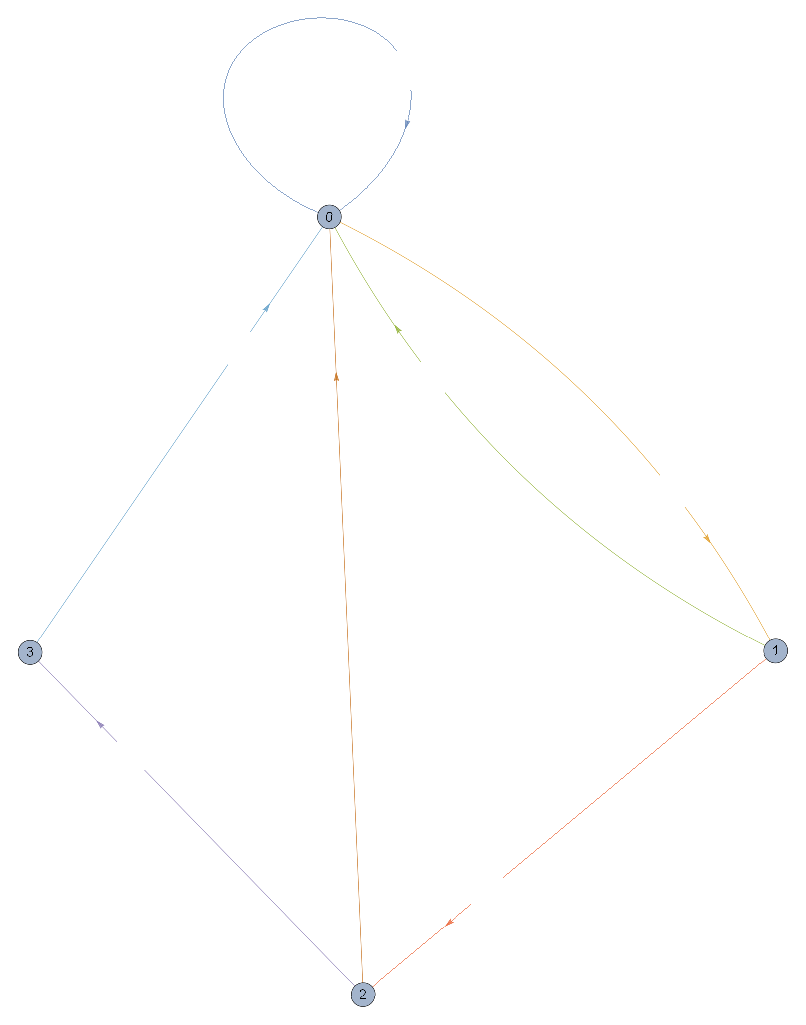
\includegraphics{doc_gr1.eps}

\subsubsection*{Image List for the first 12 Turing Machines}

\begin{doublespace}
\noindent\(\pmb{\text{imageList}=\{,,,,,,,,,,,\};}\)
\end{doublespace}

\subsubsection*{Visualization of first 12 TM}

\begin{doublespace}
\noindent\(\pmb{\text{ImageCollage}[\text{imageList}]}\)
\end{doublespace}

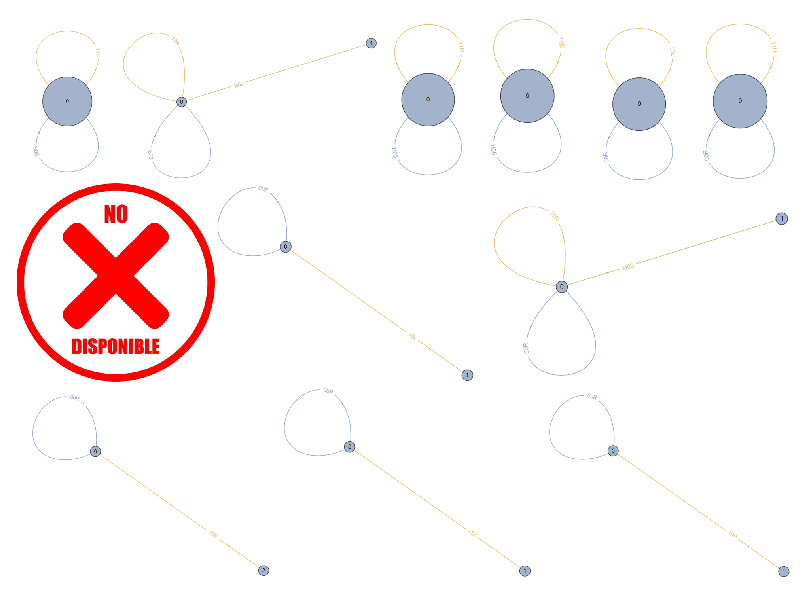
\includegraphics{doc_gr2.eps}

\begin{doublespace}
\noindent\(\pmb{\text{procesado}=\text{Table}[\{\text{(*Estado inicial*)}(\text{StringSplit}[\text{MT}[[i]],\text{{``}-$>${''}}][[1]]\text{//}\text{Characters})[[1\text{;;}-2]]\text{//}\text{StringJoin}
\text{//}\text{ToExpression},}\\
\pmb{\text{(*Valor que leo*)}(\text{StringSplit}[\text{MT}[[i]],\text{{``}-$>${''}}][[1]]\text{//}\text{Characters})\text{//}\text{Last}\text{//}\text{ToExpression},}\\
\pmb{\text{(*Valor que escribo*)}(\text{StringSplit}[\text{MT}[[i]],\text{{``}-$>${''}}][[2]]\text{//}\text{Characters})[[-2]]\text{//}\text{ToExpression},}\\
\pmb{\text{(*}\text{Movimiento}\text{*)}(\text{StringSplit}[\text{MT}[[i]],\text{{``}-$>${''}}][[2]]\text{//}\text{Characters})\text{//}\text{Last}\text{//}\text{ToExpression},}\\
\pmb{\text{(*Estado siguiente*)}(\text{StringSplit}[\text{MT}[[i]],\text{{``}-$>${''}}][[2]]\text{//}\text{Characters})[[\text{;;}-3]]\text{//}\text{StringJoin}\text{//}\text{ToExpression}}\\
\pmb{\},}\\
\pmb{\{i,1,\text{Length}[\text{MT}]\}];}\\
\pmb{\text{Export}[\text{{``}procesado.csv{''}}, \text{procesado}]}\)
\end{doublespace}

\begin{doublespace}
\noindent\(\text{procesado.csv}\)
\end{doublespace}

\begin{doublespace}
\noindent\(\pmb{\text{}}\)
\end{doublespace}

\subsection*{In order to execute the decoder for the UTM we need to introduce a number to execute \(U(n,m)=\)}

\begin{doublespace}
\noindent\(\pmb{\text{ExternalEvaluate}[\text{session},\text{File}[\text{{``}decoderTM.py{''}}]];}\\
\pmb{\text{TMexecution}=\text{ExternalEvaluate}[\text{session},\text{{``}execution{''}}];}\\
\pmb{\text{execution}=\text{TMexecution}[231];}\)
\end{doublespace}

\noindent\(\text{0 $\backslash $t 0 [1] 0 1 0 1 0 0 0 1 0 1 0 1 0 1 1 0 }\)

\noindent\(\text{1 $\backslash $t 0 0 [0] 1 0 1 0 0 0 1 0 1 0 1 0 1 1 0 }\)

\noindent\(\text{0 $\backslash $t 0 0 1 [1] 0 1 0 0 0 1 0 1 0 1 0 1 1 0 }\)

\noindent\(\text{1 $\backslash $t 0 0 1 0 [0] 1 0 0 0 1 0 1 0 1 0 1 1 0 }\)

\noindent\(\text{0 $\backslash $t 0 0 1 0 1 [1] 0 0 0 1 0 1 0 1 0 1 1 0 }\)

\noindent\(\text{1 $\backslash $t 0 0 1 0 1 0 [0] 0 0 1 0 1 0 1 0 1 1 0 }\)

\noindent\(\text{0 $\backslash $t 0 0 1 0 1 0 1 [0] 0 1 0 1 0 1 0 1 1 0 }\)

\noindent\(\text{0 $\backslash $t 0 0 1 0 1 0 1 0 [0] 1 0 1 0 1 0 1 1 0 }\)

\noindent\(\text{0 $\backslash $t 0 0 1 0 1 0 1 0 0 [1] 0 1 0 1 0 1 1 0 }\)

\noindent\(\text{1 $\backslash $t 0 0 1 0 1 0 1 0 0 0 [0] 1 0 1 0 1 1 0 }\)

\noindent\(\text{0 $\backslash $t 0 0 1 0 1 0 1 0 0 0 1 [1] 0 1 0 1 1 0 }\)

\noindent\(\text{1 $\backslash $t 0 0 1 0 1 0 1 0 0 0 1 0 [0] 1 0 1 1 0 }\)

\noindent\(\text{0 $\backslash $t 0 0 1 0 1 0 1 0 0 0 1 0 1 [1] 0 1 1 0 }\)

\noindent\(\text{1 $\backslash $t 0 0 1 0 1 0 1 0 0 0 1 0 1 0 [0] 1 1 0 }\)

\noindent\(\text{0 $\backslash $t 0 0 1 0 1 0 1 0 0 0 1 0 1 0 1 [1] 1 0 }\)

\noindent\(\text{1 $\backslash $t 0 0 1 0 1 0 1 0 0 0 1 0 1 0 1 0 [1] 0 }\)

\noindent\(\text{10 $\backslash $t 0 0 1 0 1 0 1 0 0 0 1 0 1 0 1 0 0 [0] }\)

\noindent\(\text{11 $\backslash $t 0 0 1 0 1 0 1 0 0 0 1 0 1 0 1 0 0 1 [0] }\)

\noindent\(\text{H $\backslash $t 0 0 1 0 1 0 1 0 0 0 1 0 1 0 1 0 0 1 1 [0] }\)

\subsection*{Formato posible para la visualizaci{\' o}n de las m{\' a}quinas de Turing.}

\begin{doublespace}
\noindent\(\pmb{a=\{\{0,\text{{``}[1]{''}},0,0,0,1,1,0\},}\\
\pmb{\{0,0 ,\text{{``}[0]{''}},0,0,1,1,0\},}\\
\pmb{\{0,0,1,\text{{``}[0]{''}},0,1,1,0\},}\\
\pmb{\{0,0,1,0,\text{{``}[0]{''}},1,1,0\},}\\
\pmb{\{0 ,0,1,0,0,\text{{``}[1]{''}},1,0\},}\\
\pmb{\{0,0,1,0,0,0,\text{{``}[1]{''}},0\},}\\
\pmb{\{0,0,1,0,0,0,0,\text{{``}[0]{''}}\},}\\
\pmb{\{0,0,1,0,0,0,0,1,\text{{``}[0]{''}}\},}\\
\pmb{\{0,0,1,0,0,0,0,1,1,\text{{``}[0]{''}}\}}\\
\pmb{\};}\)
\end{doublespace}

\begin{doublespace}
\noindent\(\pmb{a\text{/.}\{\text{{``}[0]{''}}\text{-$>$}\text{Pink},\text{{``}[1]{''}}\text{-$>$}\text{Green},0\text{-$>$}\text{Yellow},1\text{-$>$}
\text{Yellow}\}\text{//}\text{Grid}}\)
\end{doublespace}

\begin{doublespace}
\noindent\(\begin{array}{cccccccccc}
 \fbox{$$} & \fbox{$$} & \fbox{$$} & \fbox{$$} & \fbox{$$} & \fbox{$$} & \fbox{$$} & \fbox{$$} & \text{} & \text{} \\
 \fbox{$$} & \fbox{$$} & \fbox{$$} & \fbox{$$} & \fbox{$$} & \fbox{$$} & \fbox{$$} & \fbox{$$} & \text{} & \text{} \\
 \fbox{$$} & \fbox{$$} & \fbox{$$} & \fbox{$$} & \fbox{$$} & \fbox{$$} & \fbox{$$} & \fbox{$$} & \text{} & \text{} \\
 \fbox{$$} & \fbox{$$} & \fbox{$$} & \fbox{$$} & \fbox{$$} & \fbox{$$} & \fbox{$$} & \fbox{$$} & \text{} & \text{} \\
 \fbox{$$} & \fbox{$$} & \fbox{$$} & \fbox{$$} & \fbox{$$} & \fbox{$$} & \fbox{$$} & \fbox{$$} & \text{} & \text{} \\
 \fbox{$$} & \fbox{$$} & \fbox{$$} & \fbox{$$} & \fbox{$$} & \fbox{$$} & \fbox{$$} & \fbox{$$} & \text{} & \text{} \\
 \fbox{$$} & \fbox{$$} & \fbox{$$} & \fbox{$$} & \fbox{$$} & \fbox{$$} & \fbox{$$} & \fbox{$$} & \text{} & \text{} \\
 \fbox{$$} & \fbox{$$} & \fbox{$$} & \fbox{$$} & \fbox{$$} & \fbox{$$} & \fbox{$$} & \fbox{$$} & \fbox{$$} & \text{} \\
 \fbox{$$} & \fbox{$$} & \fbox{$$} & \fbox{$$} & \fbox{$$} & \fbox{$$} & \fbox{$$} & \fbox{$$} & \fbox{$$} & \fbox{$$} \\
\end{array}\)
\end{doublespace}

\end{document}
